\documentclass[a4paper,11pt]{article}


\usepackage{preambulo} 
 
\renewcommand{\lstlistingname}{Listado}
\lstset{
    backgroundcolor=\color[rgb]{0.86,0.88,0.93},
    language=R, keywordstyle=\color[rgb]{0,0,1},
    basicstyle=\footnotesize \ttfamily,breaklines=true,
    escapeinside={\%*}{*)}
}
\usepackage{footmisc} \renewcommand{\labelitemi}{$\circ$}
\usepackage{enumitem} \setlist[itemize]{leftmargin=*}

\usepackage{scrextend}
\deffootnote[1em]{1em}{1em}{\textsuperscript{\thefootnotemark}\,}

%%%%%%%%%% Document starts here %%%%%%%%%%%

\begin{document}
%%%%%%%%%% Title %%%%%%%%%%%
\begin{figure}[!h] 
\includegraphics [scale=0.3] {Imagens/Course-logo} \end{figure}

\begin{spacing}{1.5}
{\Large\sc \noindent Homework I} \\

{\large\sc \noindent Nome completo: Lucas de Oliveira Sobral}\\
%{\large\sc \noindent Nome completo:}\\
{\large\sc \noindent Numero de matricula: 556944}\\
%{\large\sc \noindent Numero de matricula: }\\
{\large\sc \noindent Nome completo:Álvaro José Passos de Freitas Neto}\\
%{\large\sc \noindent Nome completo:}\\
{\large\sc \noindent Numero de matricula: 567593}
%{\large\sc \noindent Numero de matricula: }
\end{spacing}

\vskip1cm

%%%%%%%%%% Content starts here %%%%%%%%%%%
\section{Questão}  \label{sec:q1}
As emissões diárias de um gás poluente de uma planta industrial foram registradas 80
vezes, em uma determinada unidade de medida. Os dados obtidos estão apresentados na
Tabela \ref{tab:ex1}:

\begin{table}[h]
    \centering
    \begin{tabular}{*{12}{c}} % Define 12 colunas centradas
        15.8 & 22.7 & 26.8 & 19.1 & 18.5 & 14.4 & 8.3 & 25.9 & 26.4 & 9.8 & 21.9 & 10.5 \\
        17.3 & 6.2 & 18.0 & 22.9 & 24.6 & 19.4 & 12.3 & 15.9 & 20.1 & 17.0 & 22.3 & 27.5 \\
        23.9 & 17.5 & 11.0 & 20.4 & 16.2 & 20.8 & 20.9 & 21.4 & 18.0 & 24.3 & 11.8 & 17.9 \\
        18.7 & 12.8 & 15.5 & 19.2 & 13.9 & 28.6 & 19.4 & 21.6 & 13.5 & 24.6 & 20.0 & 24.1 \\
        9.0 & 17.6 & 25.7 & 20.1 & 13.2 & 23.7 & 10.7 & 19.0 & 14.5 & 18.1 & 31.8 & 28.5 \\
        22.7 & 15.2 & 23.0 & 29.6 & 11.2 & 14.7 & 20.5 & 26.6 & 13.3 & 18.1 & 24.8 & 26.1 \\
        7.7 & 22.5 & 19.3 & 19.4 & 16.7 & 16.9 & 23.5 & 18.4 
    \end{tabular}
    \caption{Emissões diárias de gás poluente (questão 1).} % Legenda posicionada corretamente.
    \label{tab:ex1}
\end{table}


\begin{enumerate}[leftmargin=*]
\item Calcule as medidas de tendência central (média, mediana e moda) e as medidas de
dispersão (amplitude, variância, desvio padrão e coeficiente de variação) para o conjunto de dados da Tabela \ref{tab:ex1}.  Interprete os resultados

\item Construa um histograma e um boxplot para os dados de emissões. Os dados parecem
estar simetricamente distribuídos? Existem valores atípicos?

\item Determine os quartis (Q1, Q2, Q3) e o intervalo interquartil (IQR). Utilize esses valores
para reforçar sua análise sobre a presença de valores atípicos

\item Suponha que o limite máximo aceitável diário para as emissões seja de 25 unidades.
Qual a proporção de dias em que a planta excedeu esse limite? O comportamento
geral das emissões estaria em conformidade com esse padrão regulatório? 

\end{enumerate} 


\subsection*{Solução da questão} 			

\subsubsection*{Descrição da atividade}
A questão 1 visa exercitar os conceitos de estatística descritiva como distribuição de frequência, medidas de tendência central, medidas de dispersão e gráficos básicos para análise de 80 dados, sendo estes, emissões de um gás poluente de uma indústria. 

\subsubsection*{Distribuição de frequência - Base Teórica:} 

\begin{itemize}
\item[]

\text{\large Classes ou valores (\(x_i\))}
    \item São diferentes valores que  a variável assume ou intervalos (classes) em que os dados são agrupados.

\text{\large Frequência Absoluta (\(n_i\))}
    \item A frequência absoluta o número de vezes que um determinado valor ou intervalo de valores aparece em um conjunto de dados. A soma de todas as frequências absolutas deve ser igual ao número total de observações (N)

    \[\sum n_i = N\]

\text{\large Frequência Relativa (\(f_i\))}
    \item A frequência relativa é a proporção de observações pertencentes ao valor (Xi) em relação ao total de observações.

    \[f_i = \frac{ni}{N}\]

\text{\large Frequência Percentual (\(p_i\))}
    \item É a frequência relativa multiplicada por 100, deixando o dado em forma de porcentagem.

    \[p_i = f_i * 100\]

\text{\large Frequência Acumulada (\(N_i\))}
    \item É a soma das frequências absolutas de 1 até o valor $x_i$. Serve para mostrar o total de observações que possuem um valor menor ou igual ao limite superior da classe.

    \[N_i = \sum_{j=1}^{i} n_j = n_1 + n_2 + ... + n_i\]

\text{\large Frequência Relativa Acumulada (\(F_i\))}
    \item É a soma das frequências relativas de 1 até o valor $x_i$. Serve para mostrar o total de observações que possuem um valor menor ou igual ao limite superior da classe.

    \[F_i = \sum_{j=1}^{i} f_j = f_1 + f_2 + ... + f_i\]

\text{\large Frequência Percentual Acumulada (\(P_i\))}
    \item É a soma das frequência percentuais de 1 até o valor $x_i$.

    \[P_i = \sum_{j=1}^{i} p_j = p_1 + p_2 + ... + p_i\]

\end{itemize}

\subsubsection*{Medidas de tendência central - Base Teórica:} 

\begin{itemize}
\item[]

\text{\large Moda (\(M_o\))}
    \item É o valor que ocorre com maior frequência em um conjunto de dados. Um conjunto de dados pode ter nenhum valor que se destaque sendo assim ele não tem moda (amodal), pode ter uma moda (unimodal), duas modas quando dois valores se destacam (bimodal) ou várias modas quando vários valores se destacam(polimodal).


\text{\large Mediana (\(M_d\))}
    \item É o valor que ocupa a posição central em um conjunto de dados ordenados de forma crescente ou decrescente, para obter a mediana de um conjunto ímpares de dados devemos pegar o total de dados somar um e dividir por dois, para dados pares devemos pegar os dois do meio e fazer a média dos dois, dividindo por dois.

    \item Para conjunto ímpar \[M_d = \frac{N+1}{2}\]
    \item Para conjunto par \[M_d = \frac{x_{\frac{N}{2}} + x_{(\frac{N}{2} + 1)}}{2}\]


\text{\large Mediana para dados agrupados (\(M_d\))}
    \item Para dados agrupados onde não sabemos com exatidão os valores de $x_i$, dessa forma devemos utilizar a frequência acumulada $N_i$ para saber em qual intervalo fica a mediana, após isso precisaremos utilizar a seguinte fórmula:

    \[M_d = L_i + \frac{\frac{N}{2} - N_i }{n_i} * h\]

    Onde:
    \item $L_i$: Limite inferior da classe da mediana.
    \item $\frac{N}{2} ou \sum fi$: Somatório da frequência absoluta.
    \item $N_i$: Frequência acumulada da classe anterior à mediana.
    \item $h$: Amplitude do intervalo da classe da mediana.
    \item $n_i$: Frequência absoluta da classe.



\text{\large Média Aritmética(\(\overline{x}\))}
    \item É a soma de todos os valores do conjunto de dados dividida pelo número total de dados.

    \[\overline{x} = \frac{\sum x_i}{N}\]

\text{\large Média Aritmética Ponderada(\(\overline{x}_w\))}
    \item É utilizada quando os valores do conjunto de dados não tem a mesma importância ou peso. Em vez de cada valor contribuir igualmente para o cálculo da média, cada um é multiplicado pelo peso $w_i$.

    \[\overline{x}_w = \frac{\sum(x_i*w_i)}{\sum w_i}\]


\text{\large Média Ponderada para dados agrupados por intervalo(\(\overline{x}_a\))}
    \item Para dados agrupados devemos fazer o somatório de $x_m$ (média do intervalo) com a multiplicação da frequência absoluta $n_i$ e dividir pelo total de valores $N$.

    \[\overline{x}_a = \frac{\sum(x_m * n_i)}{N}\]

    \item onde $x_m = \frac{L_{inferior} + L_{superior}}{2}$


\end{itemize}

\subsubsection*{Medidas de dispersão - Base Teórica:} 
\begin{itemize}
\item[]

\text{\large Dispersão}
    \item É a medida que informa o quão espalhados estão os dados do centro, temos quatro principais formas de calcular dispersão:

\text{\large Amplitude(A)}
    \item Corresponde à diferença entre o maior e o menor valor do conjunto de dados. É muito sensível a valores extremos (outliers).

     \[ A = \text{Valor}_{\text{máximo}} -\text{Valor}_{\text{mínimo}} \]
    
\text{\large Variância($\sigma^2$ ou $S^2$ )}
    \item Em suma é a média dos quadrados das distâncias de cada valor em relação à média, ele fornece uma medida numérica da dispersão, sendo um valor alto indicando que os dados estão muito espalhados em relação à média (pouca homogeneidade), enquanto um valor baixo indica que os dados estão próximos à média (muita homogeneidade). 

    \[\sigma^2 = \frac{\sum (x_i - \overline{x})^2}{N}\]

    \item ou simplesmente o somatório do desvio médio ao quadrado.

    \[\sigma^2 = \frac{\sum (dm_i{^2})}{N}\]

    sendo 
    \[dm = \frac{\sum (desvio_i)}{N}\] 

    \[desvio_i = \overline{x} - x_i\]

    \item Observação: substituir $N$ por $N-1$ no denominador fornece uma estimativa não enviesada da verdadeira variância da população e transformando em uma fórmula para variância amostral.

    \[S^2 = \frac{\sum (x_i - \overline{x})^2}{N-1}\]

\text{\large Desvio padrão($\sigma$ ou $S$ )}
    \item É a raiz quadrada da variância e serve para retornar à unidade da medida original. 

    \[\sigma = \sqrt {\sigma^2} = \sqrt{\frac{\sum (x_i - \overline{x})^2}{N}}\]

\text{\large Coeficiente de Variação (CV)}
    \item É uma medida de dispersão relativa, expressa como uma porcentagem. É a razão entre o desvio padrão e a média. Sua principal utilidade é comparar a variabilidade de dois ou mais conjuntos de dados que possuem médias ou unidades de medida diferentes. Um CV baixo indica baixa variabilidade relativa, enquanto um CV alto indica alta variabilidade relativa.

    \[ CV = \frac{S}{\overline{x}} \times 100\% \]

    Onde:
    \item $S$: Desvio padrão da amostra.
    \item $\overline{x}$: Média da amostra.


\end{itemize}

\subsubsection*{Gráficos - base teórica} 

\begin{itemize}
\item[]
\text{\large Histograma}
    \item É um gráfico de barras que representa a distribuição de frequências de um conjunto de dados, ele mostra como os valores se distribuem ao longo de intervalos (chamados de classes).

\vspace{5mm} %5mm vertical space

    Onde:
    \item O eixo x tem os intervalos de valores (classes).
    \item O eixo x tem as frequências.
    
\vspace{5mm} %5mm vertical space

    Funcionalidade:
    \item É um gráfico utilizado para representar dados quantitativos (sejam discretos ou contínuos), ou seja, valores numéricos que podem ser contados ou medidos, sua principal funcionalidade é mostrar de forma visual como os dados estão distribuídos, permitindo identificar padrões, tendências centrais, dispersão e possíveis outliers (valores fora do comum).

\vspace{5mm} %5mm vertical space

    Exemplo (Retirado do slides):
    \begin{figure}[!h] 
        \centering
        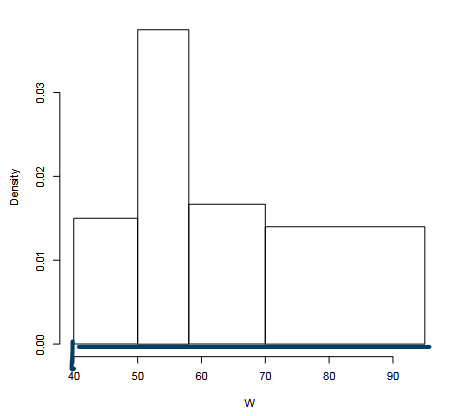
\includegraphics [scale=0.5] {Imagens/Graficos/histograma_exemplo} 
    \end{figure}
    
\text{\large Boxplot}
    \item É um gráfico utilizado para representar a distribuição de dados quantitativos, ele é construído com base em alguns valores estatísticos principais.

\vspace{5mm} %5mm vertical space

    São eles:
    \item Numero total de amostras (n).
    \item Mínimo.
    \item Primeiro quartil (Q1) (25\% dos dados estão abaixo dele).
        \[Q1 = \frac{1}{4} \times (n + 1) \]
    \item Mediana (Q2) (50\% dos dados estão abaixo dele) (mediana).
        \[Q2 = \frac{2}{4} \times (n + 1) = \frac{n + 1}{2}\]
    \item Terceiro quartil (Q3) (75\% dos dados estão abaixo dele).
        \[Q3 = \frac{3}{4} \times (n + 1)\]
    \item Máximo.

As fórmulas do primeiro e do terceiro quartil retornam a posição deles. Se for um inteiro, pegue o valor na posição se não for inteiro pegue os valores acima e abaixo da posição e faça a média deles.

\vspace{5mm} %5mm vertical space

    Com base neles calcula-se o IQR e os limites (inferior e superior):

    \item IQR.
        \[IQR = Q3 - Q1\]
    \item Limite inferior.
        \[\text{Limite inferior} = Q1 - 1.5 \times IQR\]
    \item Limite superior.
        \[\text{Limite superior} = Q3 + 1.5 \times IQR\]

    Valores que estiverem fora desses limites são considerados \textbf{outliers}, ou valores atípicos.
    
\vspace{5mm} %5mm vertical space

    Funcionalidade:
    \item É utilizado para observar a distribuição dos dados, a tendência central e a dispersão dentro de um conjunto amostral, principalmente para facilitar a visualização da variabilidade e da simetria dos dados, bem como identificar valores extremos e comparar distribuições entre diferentes grupos ou amostras.

\vspace{5mm} %5mm vertical space

    Exemplo (Retirado do slides):
    \begin{figure}[!h] 
        \centering
        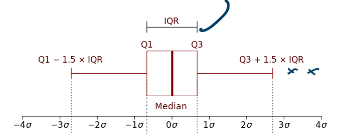
\includegraphics [scale=0.8] {Imagens/Graficos/boxplot-exemplo} 
    \end{figure}

\end{itemize}

\begin{description}

\item \textbf{[1.1] Resposta}:

\textbf{Média}

Temos 80 dados e um somatório deles utilizando calculadora:
\item primeira Linha: 220.1
\item segunda Linha: 223.5
\item terceira Linha: 224.1
\item quarta Linha: 231.9
\item quinta Linha: 231.9
\item sexta Linha: 245.8
\item sétima Linha: 144.4

Somando todas as linhas: 1521.7

média dos gases poluentes emitidos diariamente: 
\[\overline{x} = \frac{\sum x_i}{N} = \frac{1521.7}{80} = 19.02125\]

Sendo o valor encontrado sendo o mesmo calculado pelo R.

\begin{lstlisting}
    > mediaGases = media(gases) # usando funcao propria
    > mediaGases
    [1] 19.02125
    > print(mean(gases)) # usando funcao padrao do R
    [1] 19.02125
    \end{lstlisting}

\textbf{Mediana}:
Mediana de conjunto par pode ser encontrada ordenando os dados e aplicando a fórmula da mediana:


\begin{table}[H]
    \centering
    \begin{tabular}{cccccccccc}
        \hline
        6.2 & 7.7 & 8.3 & 9.0 & 9.8 & 10.5 & 10.7 & 11.0 & 11.2 & 11.8 \\
        12.3 & 12.8 & 13.2 & 13.3 & 13.5 & 13.9 & 14.4 & 14.5 & 14.7 & 15.2 \\
        15.5 & 15.8 & 15.9 & 16.2 & 16.7 & 16.9 & 17.0 & 17.3 & 17.5 & 17.6 \\
        17.9 & 18.0 & 18.0 & 18.1 & 18.1 & 18.4 & 18.5 & 18.7 & 19.0 & 19.1 \\
        19.2 & 19.3 & 19.4 & 19.4 & 19.4 & 20.0 & 20.1 & 20.1 & 20.4 & 20.5 \\
        20.8 & 20.9 & 21.4 & 21.6 & 21.9 & 22.3 & 22.5 & 22.7 & 22.7 & 22.9 \\
        23.0 & 23.5 & 23.7 & 23.9 & 24.1 & 24.3 & 24.6 & 24.6 & 24.8 & 25.7 \\
        25.9 & 26.1 & 26.4 & 26.6 & 26.8 & 27.5 & 28.5 & 
        28.6 & 29.6 & 31.8 \\
        \hline
    \end{tabular}
    \caption{Emissões diárias de gás poluente ordenados com R (questão 1).}
    \label{tab:q1}
\end{table}

Ordenei os dados utilizando R pois eram muitos valores, com base na tabela ordenada pude achar os índices 40 e 41 e aplicar a fórmula da mediana que deu valor de (19.15). Sendo o valor encontrado sendo o mesmo calculado pelo R. 
\[M_d = \frac{x_{\frac{N}{2}} + x_{(\frac{N}{2} + 1)}}{2} \xrightarrow{} \frac{x_{40} + x_{41}}{2}  = \frac{19.1 + 19.2}{2} = 19.15\]

\begin{lstlisting}
    > medianaGases = mediana(gases_ordenados) # usando funcao propria
    > medianaGases
    [1] 19.15
    > print(median(gases_ordenados)) # usando funcao padrao do R
    [1] 19.15
    \end{lstlisting}
 
\textbf{Moda}: 19.4 pois é o que mais se destaca com 3 repetições. Sendo o valor encontrado sendo o mesmo calculado pelo R.

\begin{lstlisting}
    > modaGases = moda(gases_ordenados)
    > modaGases
    [1] 19.4
\end{lstlisting}

\textbf{Amplitude}: É o maior valor subtraído do menor valor do conjunto de dados. Sendo o valor encontrado sendo o mesmo calculado pelo R.
\[ A = \text{Valor}_{\text{máximo}} -\text{Valor}_{\text{mínimo}} \]
\[A = 31.8 - 6.2 = 25.6\]

\textbf{Variância}: \[\sigma^2 = \frac{\sum (x_i - \overline{x})^2}{N}\]

Tabela de desvio ($x_i - \overline{x}$:
\begin{table}[H]
    \centering
    % Define 9 colunas centradas
    \begin{tabular}{ccccccccc}
        \hline
        -12.821 & -11.321 & -10.721 & -10.021 & -9.221 & -8.521 & -8.321 & -8.021 & -7.821 \\ 
        -7.221 & -6.721 & -6.221 & -5.821 & -5.721 & -5.521 & -5.121 & -4.621 & -4.521 \\ 
        -4.321 & -3.821 & -3.521 & -3.221 & -3.121 & -2.821 & -2.321 & -2.121 & -2.021 \\ 
        -1.721 & -1.521 & -1.421 & -1.121 & -1.021 & -1.021 & -0.921 & -0.921 & -0.621 \\ 
        -0.521 & -0.311 & -0.021 & 0.078 & 0.178 & 0.278 & 0.378 & 0.378 & 0.378 \\ 
        0.978 & 1.078 & 1.078 & 1.378 & 1.478 & 1.778 & 1.878 & 2.378 & 2.578 \\ 
        2.878 & 3.278 & 3.478 & 3.678 & 3.678 & 3.878 & 3.978 & 4.478 & 4.678 \\ 
        4.878 & 5.078 & 5.278 & 5.578 & 5.578 & 5.778 & 6.678 & 6.878 & 7.078 \\ 
        7.378 & 7.578 & 7.778 & 8.478 & 9.478 & 9.578 & 10.578 & 12.778 \\ 
        \hline
    \end{tabular}
    \caption{Desvio das Emissões diárias de gás poluente ordenados (questão 1).}
    \label{tab:q1}
\end{table}

Agora que temos os desvios, podemos elevar cada um ao quadrado e fazer o somatório deles.

\item Primeira linha: 860.28117
\item Segunda linha: 305.385369
\item terceira linha: 87.712169
\item quarta linha: 12.718169
\item quinta linha: 0.912307
\item sexta linha: 26.353156
\item sétima linha: 130.97955
\item oitava linha: 362.35924
\item nona linha: 700.976672

Após isso aplicamos na fórmula da variância:

\[\sigma^2 = \frac{\sum 2,487.6777802}{80-1} = 31.489\]

O valor calculado pela função em R foi 30.84144, divergindo com o calculado pela calculadora, provavelmente erro de cálculo humano.

\begin{lstlisting}
    > varianciaGases = variancia(gases,mediaGases)
    > varianciaGases
    [1] 30.84144
\end{lstlisting}

Diferença percentil:

\[Erro_{percentil} = \frac{|30.84144 - 31.489|}{30.84144} * 100 \approx   2.099\% \]

\textbf{Desvio padrão}: Para o desvio padrão aplicas somente a raiz quadrada da variância, utilizando N-1 para evitar viés.
\[\sigma = \sqrt{31.489} = 5.6115\]

\begin{lstlisting}
    > desvioPadraoGases = desvioPadrao(varianciaGases)
    > desvioPadraoGases
    [1] 5.553507
\end{lstlisting}

O valor encontrada divergiu do apresentado pela função em R já que a variância também apresenta erro de 2.099\%. O desvio padrão apresentado pelo R foi 5.553507. Temos então que o erro percentil foi:

\[Erro_{percentil} = \frac{|5.553507 - 5.6115|}{5.553507} * 100 \approx   1.044\%\]

\textbf{Coeficiente de variação}: Utilizando a fórmula o valor apresentado pela calculadora foi de 162.142\%, sendo o mesmo calculado pela função em R.

 \[ CV = \frac{30.84144}{19.02125} \times 100\%  = 162.142\%\]

\begin{lstlisting}
    coeficienteVariacao <- function(variancia,media){
  return((variancia/media) * 100);
}


    > CoeficienteVGases = coeficienteVariacao(varianciaGases,mediaGases)
    > CoeficienteVGases
    [1] 162.142
\end{lstlisting}

\textbf{\item[1.2] Resposta}:

\textbf{Histograma}: Utilizando da ordenação feita na questão anterior podemos separar os dados em classes.

\vspace{5mm} %5mm vertical space

As classes que eu escolhi foram:
\begin{itemize}
    \item (5, 10]
    \item (10, 15]
    \item (15, 20]
    \item (20, 25]
    \item (25, 30]
    \item (30, 35]
\end{itemize}

\vspace{5mm} %5mm vertical space

Para melhor clareza na visualização dos dados, ao invés de usar a frequência diretamente, estarei usando a densidade, calculada da seguinte forma.

\begin{itemize}
    \item $f_i$ = frequência absoluta da classe
    \item $n$ = número total de observações
    \item $h_i$ = largura do intervalo da classe
\end{itemize}

\[d_i = \frac{f_i}{n \cdot h_i}\]

\vspace{5mm} %5mm vertical space

Fazendo a contagem de itens em cada classe usando R temos:

\begin{itemize}
    \item (5, 10] = 5
    \item (10, 15] = 14
    \item (15, 20] = 27
    \item (20, 25] = 23
    \item (25, 30] = 10
    \item (30, 35] = 1
\end{itemize}

Tendo em mente que a largura de todos os intervalos é a mesma e igual a 5 e que temos um total de 80 amostras, encontremos então a densidade usando a formula proposta.

\begin{itemize}
    \item (5, 10]:
        \[d = \frac{5}{80 \cdot 5} = 0,0125 \]
    \item (10, 15]:
        \[d = \frac{14}{80 \cdot 5} = 0,035 \]
    \item (15, 20]:
        \[d = \frac{27}{80 \cdot 5} = 0,0675 \]
    \item (20, 25]:
        \[d = \frac{23}{80 \cdot 5} = 0,0575 \]
    \item (25, 30]:
        \[d = \frac{10}{80 \cdot 5} = 0,025 \]
    \item (30, 35]:
        \[d = \frac{1}{80 \cdot 5} = 0,0025 \]
\end{itemize}

Com isso eu usei o R para criar o histograma.

    \begin{figure}[H] 
        \centering
        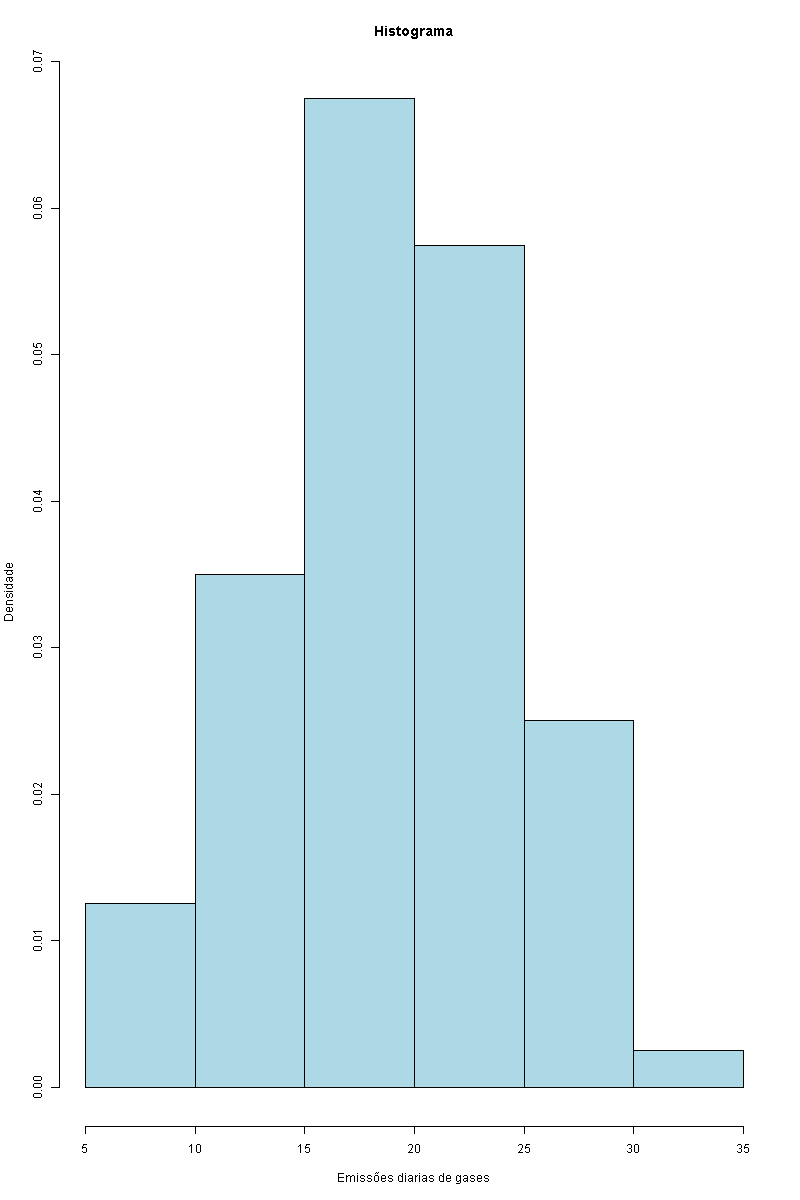
\includegraphics [scale=0.3] {Imagens/Graficos/histograma-questao1} 
    \end{figure}

\begin{lstlisting}
    > hist(gases_ordenados, 
+      probability = TRUE,   // Converte frequencia em densidade
+      col = "lightblue",    // Cor das barras
+      border = "black",     // Cor da borda
+      main = "Histograma", 
+      xlab = "Emissoes diarias de gases", 
+      ylab = "Densidade")
\end{lstlisting}

Note que os valores apontados no gráfico confirmam nossos cálculos anteriores.



\vspace{5mm} %5mm vertical space

A partir da análise do gráfico, pode-se concluir que a emissão diária de gases poluentes da fábrica costuma se concentrar entre 15 a 25 unidades, apresentando uma leve assimetria à direita e poucos dias com emissões extremas. Essa distribuição indica que, em geral, a fábrica é bem regular na quantidade de emissão de gases, porém, pela presença de alguns valores extremos, é importante verificar o que causou eles.

\textbf{boxplot}: Para criar o gráfico, deve-se levantar alguns dados inicialmente (usaremos a tabela ordenada adquirida no primeiro item).

Com isso eu usei o R para criar o boxplot.

    \begin{figure}[H] 
        \centering
        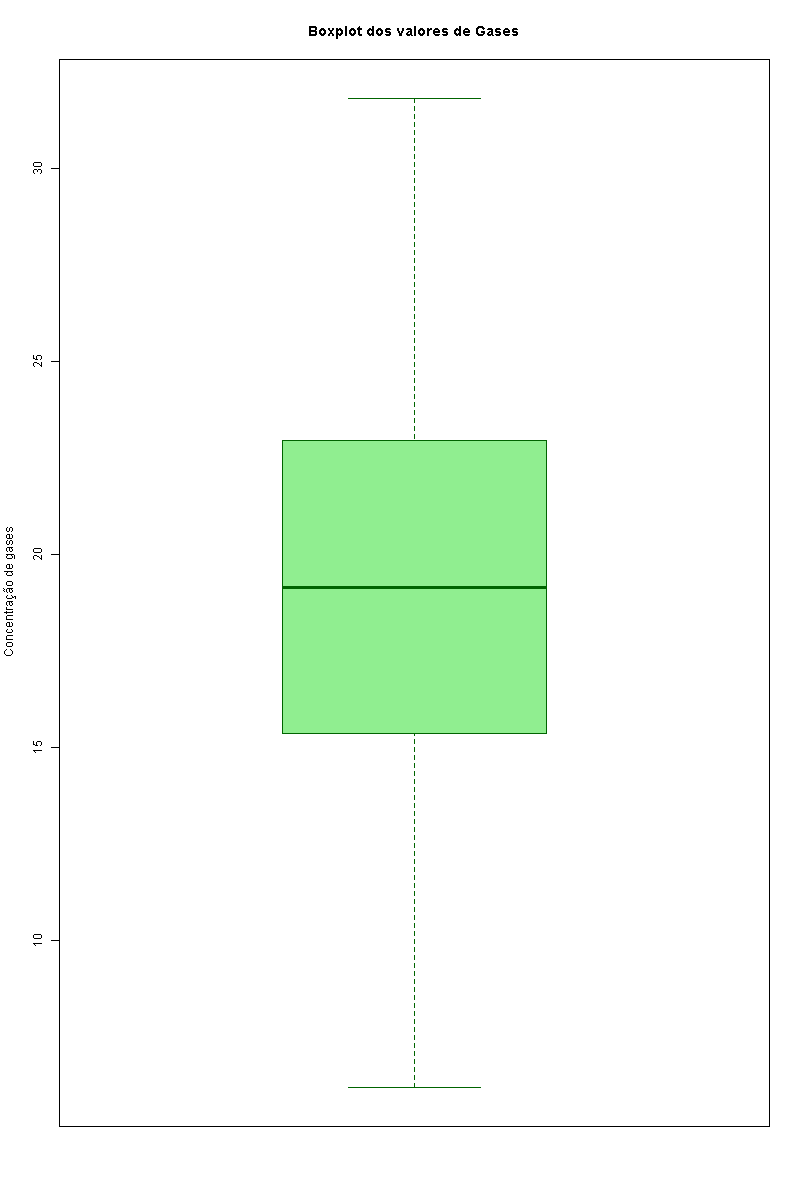
\includegraphics [scale=0.3] {Imagens/Graficos/boxplot-questao1} 
    \end{figure}


\begin{lstlisting}
    boxplot(gases_ordenados,
        main = "Boxplot dos valores de Gases",
        ylab = "Concentracao de gases",
        col = "lightgreen",
        border = "darkgreen")  
\end{lstlisting}

\vspace{5mm} %5mm vertical space

O gráfico ilustra que a fábrica emite uma quantidade consistente de poluentes na maioria dos dias, mantendo um padrão que geralmente fica entre 15 e 25 unidades.
A distribuição concentrada indica um controle razoável das emissões, apesar de haver alguns casos de emissões elevadas que merecem uma investigação (mas não são considerados outliers).

\vspace{5mm} %5mm vertical space

Portanto analisando os dois gráficos nota-se que os dados fornecidos possuem valores extremos, porem nenhum valor atípico (nenhum outlier).

\textbf{\item[1.3] Resposta}: \\

O valor mínimo e máximo já foram adquiridos no primeiro item dessa questão, além de também ter sido calculada já a mediana.

\begin{itemize}
    \item Mínimo = 6.2
    \item Máximo = 31.8
    \item Mediana = 19.15
\end{itemize}

Sabendo que temos um total de 80 amostras definirei os quartis:

\begin{itemize}
    \item Primeiro quartil (Q1) (25\% dos dados estão abaixo dele).
        \[Q1 = \frac{1}{4} \times (80 + 1) = 20.25 \]
    Como o valor não é um inteiro pegarei o valor acima (15.5) e o valor logo abaixo (15.2) e farei a media entre eles.
        \[Q1 = \frac{15.5 + 15.2}{2} = 15.35 \]
        
    \item Segundo quartil (Q2) (mediana) = 19.15
 
    \item Terceiro quartil (Q3) (75\% dos dados estão abaixo dele).
        \[Q3 = \frac{3}{4} \times (80 + 1) = 60.75\]
    Como o valor não é um inteiro pegarei o valor acima (23.0) e o valor logo abaixo (22.9) e farei a media entre eles.
        \[Q1 = \frac{23 + 22.9}{2} = 22.95 \]
\end{itemize}

Por fim com os quartis definidos calcula-se o IQR e os limites inferiores e superiores.

\begin{itemize}
    \item IQR.
        \[IQR = Q3 - Q1 = 22.95 - 15.35 = 7.6\]
    \item Limite inferior.
        \[\text{Limite inferior} = Q1 - 1.5 \times IQR = 15.35 - 1.5  \times 7.6 = 3.95\]
    \item Limite superior.
        \[\text{Limite superior} = Q3 + 1.5 \times IQR = 22.95 + 1.5 \times 7.6 = 34.35\]
\end{itemize}

\begin{lstlisting}
> quantile(gases_ordenados)
    0%    25%    50%    75%   100% 
 6.200 15.425 19.150 22.925 31.800 
\end{lstlisting}

Note que os valores calculados manualmente e pelo R confirmam a não existência de valores atípicos.

\textbf{\item[1.4] Resposta}: \\  

O histograma e o boxplot das emissões diárias de gases poluentes indicam que a maior parte dos valores se concentra entre 15 e 25 unidades, faixa em que ocorrem as emissões mais frequentes e estáveis da fábrica. A distribuição é unimodal e levemente assimétrica à direita, o que demonstra que há predominância de dias com emissões moderadas e poucos casos de valores mais altos. Essa concentração central sugere que o processo produtivo apresenta bom controle ambiental, com variações relativamente pequenas ao longo do tempo.

Considerando que o limite máximo aceitável é de 25 unidades, foi observado que 11 dos 80 dias (cerca de 13,75\%) ultrapassaram esse valor. Portanto, embora a maioria das medições (86,25\%) esteja dentro dos padrões estabelecidos, o comportamento das emissões não está totalmente em conformidade com o padrão regulatório. Esses excessos pontuais podem estar relacionados a picos de produção ou falhas no sistema de controle, indicando a necessidade de monitoramento contínuo e ajustes operacionais para garantir a plena adequação ambiental.

\end{description}

\section{Questão} \label{sec:q2}
Uma empresa italiana recebeu 20 currículos de cidadãos italianos e estrangeiros na seleção
de pessoal qualificado para o cargo de gerente de relações exteriores. A tabela \ref{tab_2} reporta as
informações consideradas relevantes na seleção: a idade, a nacionalidade, o nível mínimo
de renda desejada (em milhares de euros), os anos de experiência no trabalho

\begin{table}[H]
    \centering
    \label{tab_2}
    \begin{tabular}{c l l c c}
        \toprule
        & \textbf{Idade} & \textbf{Nacionalidade} & \textbf{Renda} & \textbf{Experiência} \\
        \midrule
        1 & 28 & Italiana & 2.3 & 2 \\
        2 & 34 & Inglesa & 1.6 & 8 \\
        3 & 46 & Belga & 1.2 & 21 \\
        4 & 26 & Espanhola & 0.9 & 1 \\
        5 & 37 & Italiana & 2.1 & 15 \\
        6 & 29 & Espanhola & 1.6 & 3 \\
        7 & 51 & Francesa & 1.8 & 28 \\
        8 & 31 & Belga & 1.4 & 5 \\
        9 & 39 & Italiana & 1.2 & 13 \\
        10 & 43 & Italiana & 2.8 & 20 \\
        11 & 58 & Italiana & 3.4 & 32 \\
        12 & 44 & Inglesa & 2.7 & 23 \\
        13 & 25 & Francesa & 1.6 & 1 \\
        14 & 23 & Espanhola & 1.2 & 0 \\
        15 & 52 & Italiana & 1.1 & 29 \\
        16 & 42 & Alemã & 2.5 & 18 \\
        17 & 48 & Francesa & 2.0 & 19 \\
        18 & 33 & Italiana & 1.7 & 7 \\
        19 & 38 & Alemã & 2.1 & 12 \\
        20 & 46 & Italiana & 3.2 & 23 \\
        \bottomrule
    \end{tabular}
        \caption{Informações na seleção da empresa italiana (questão 2).}
\end{table}

\begin{enumerate}[leftmargin=*]
\item Calcule a média, mediana e desvio padrão para as variáveis idade, renda desejada e
anos de experiência. O que você pode inferir a partir desses valores sobre o perfil típico dos candidatos?

\item  Agrupe os candidatos por nacionalidade e calcule a renda média desejada e os anos
médios de experiência para cada grupo. Qual nacionalidade apresenta a maior renda
média desejada? Qual grupo aparenta ser o mais experiente?

\item Existe correlação entre anos de experiência e renda desejada? Utilize ferramentas visuais apropriadas (por exemplo, gráfico de dispersão) e calcule o coeficiente de correlação
de Pearson. Interprete o resultado

\item Suponha que a empresa queira priorizar candidatos com pelo menos 10 anos de experiência e renda desejada inferior a 2,0 (mil euros). Quantos candidatos atendem a ambos
os critérios? Liste suas nacionalidades e idades

\item Construa gráficos que permitam visualizar a distribuição da idade e da renda desejada,
separados por nacionalidade. Utilize histogramas, box-plots ou gráficos de barras, e
comente as principais diferenças observadas entre os grupos

\end{enumerate}

\subsection*{Solução da questão} 		

\subsubsection*{Descrição da atividade}
Esta atividade exercita novamente os conceitos básicos de estatística descritiva, porém, com ênfase maior no cálculo e no gráfico de correlação entre variáveis de uma base de dados de vinte currículos e diferentes níveis de variáveis como, idade, nacionalidade, renda desejada e experiência no trabalho de relações exteriores.

\subsubsection*{Medidas de dispersão - Base Teórica:} 

\begin{itemize}
\item[]

\text{\large Coeficiente de variação de Pearson ($r_{xy)}$}
    \item É uma medida estatística que descreve o grau e a direção da associação linear entre duas variáveis quantitativas (X e Y).

    \[r_{xy} = \frac{\sum{(x_i - \overline{x})(y_i-\overline{y})}}{\sqrt{\sum (x_i - \overline{x})^2 \sum(y_i-\overline{y})^2}}\]

    O resultado estará em um intervalo de [-1,1], 

\end{itemize}

\subsubsection*{Gráficos(base teórica)} 

\begin{itemize}
\item[]

\text{\large Gráfico de dispersão}
    \item O Gráfico de Dispersão é uma representação gráfica de duas variáveis quantitativas, $X$ e $Y$, onde cada ponto no gráfico corresponde a um par de valores $(x_i, y_i)$ de uma observação.

    Com ele podemos:
    \item Verificar a Direção:
    \begin{itemize}
        \item Positiva: Os pontos tendem a subir da esquerda para a direita.
        \item Negativa: Os pontos tendem a descer da esquerda para a direita.
    \end{itemize}
    
    \item Avaliar a Força (Correlação):
    \begin{itemize}
        \item Forte: Os pontos estão muito agrupados e próximos a uma linha imaginária (ou à linha de regressão).
        \item Fraca: Os pontos estão muito espalhados, formando uma nuvem difusa.
    \end{itemize}
    
    \item Checar a Forma:
    \begin{itemize}
        \item Linear: Os pontos formam uma linha reta. (O coeficiente de Pearson $r$ só mede este tipo de relação).
        \item Não Linear (Curvilínea): Os pontos formam uma curva (ex: parábola).
        \item Nenhuma: Os pontos estão distribuídos aleatoriamente.
    \end{itemize}    
    
    \item Identificar Outliers:
    \begin{itemize}
        \item Pontos que se afastam significativamente da tendência geral dos outros pontos. Eles podem distorcer o cálculo da Média, Variância e, principalmente, do Coeficiente de Correlação ($r$).
    \end{itemize}

    \item Exemplo de gráficos de correlação:

    \begin{figure}[H] 
    \centering 
    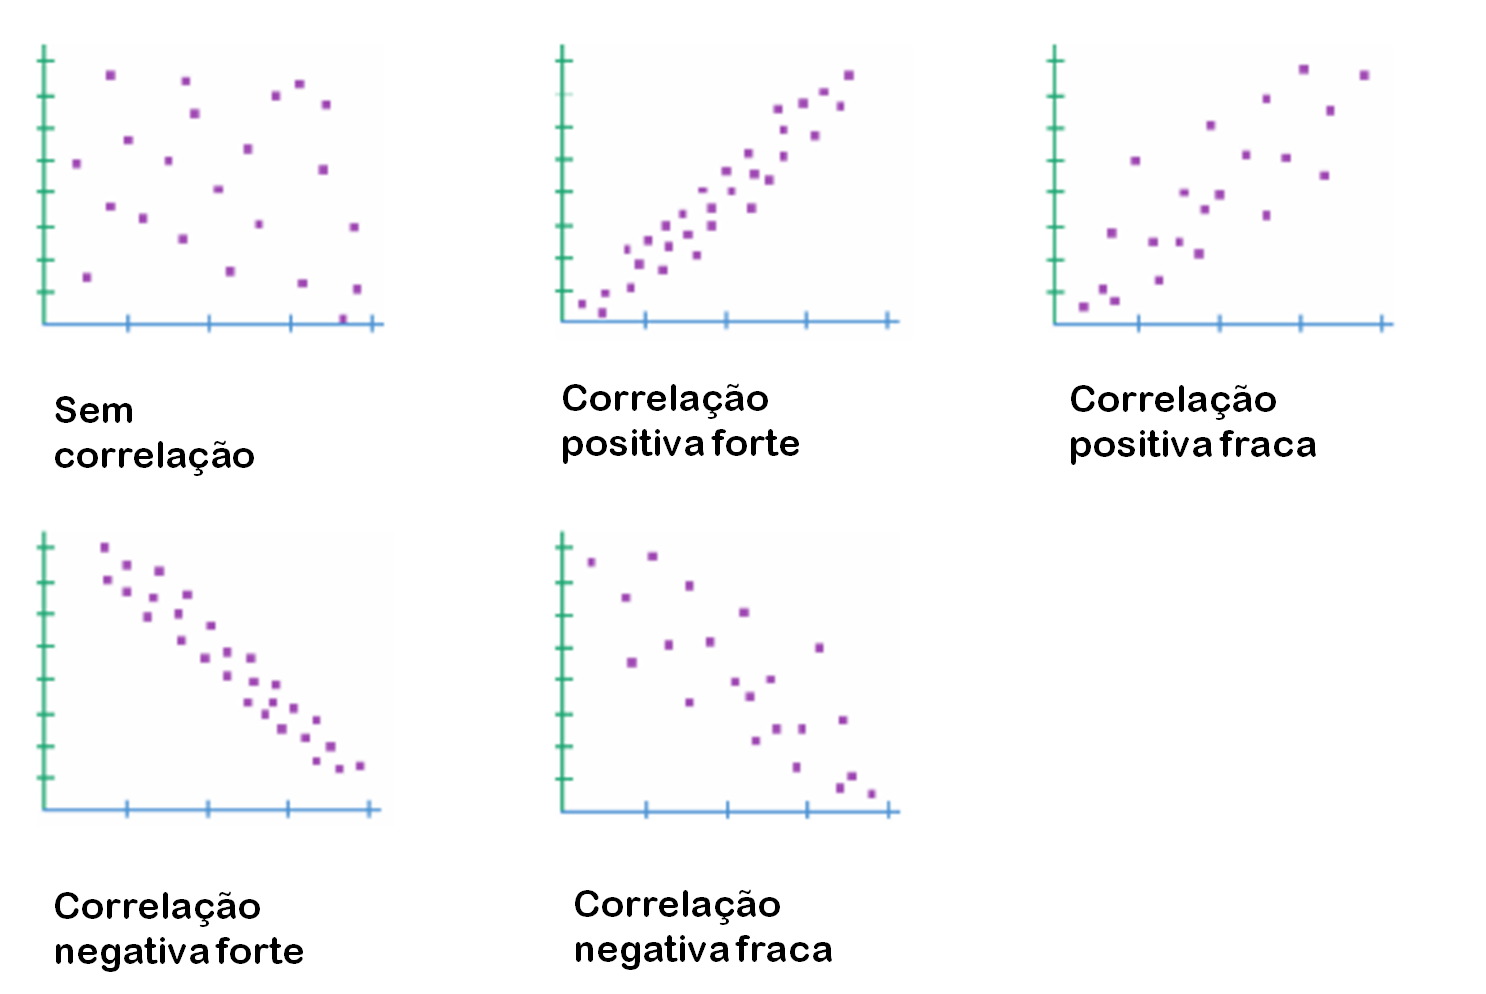
\includegraphics[width=0.8\textwidth]{Imagens/Graficos/Graficos de correlacao.png} 
\end{figure}

    
\end{itemize}



\begin{description}[leftmargin=*]

\item[2.1] \textbf{Resposta}:

\item \textbf{Idade}: \\
Média:
Somando todos os valores de idade e dividindo pelo total de números obtemos uma média igual ao R.
\[\overline{x}_{idade} = \frac{773}{20} = 38.65\]

\begin{lstlisting}
> mediaIdade = media(curriculos$Idade....idade);
> mediaIdade
[1] 38.65
> mean(curriculos$Idade....idade)
[1] 38.65    
\end{lstlisting}

Mediana:
Ordenando de maneira crescente as idades usando R:

$Idade: 23, 25, 26, 28, 29, 31, 33, 34, 37, 38, 39, 42, 43, 44, 46, 46, 48, 51, 52, 58$

Mediana obtida igual ao R.
\[Md_{idade} = \frac{X_{10}+X_{11}}{2} = \frac{38+39}{2} =38.5\]

\begin{lstlisting}
> medianaIdade = mediana(curriculos$Idade....idade);
> medianaIdade
[1] 38.5
> median(curriculos$Idade....idade)
[1] 38.5
\end{lstlisting}

Desvio Padrão:
O desvio padrão calculado após a tabela de desvios e cada um elevado ao quadrado, depois somado e dividido por 19.
\begin{table}[H]
    \centering
    \begin{tabular}{cccccccccc}
        \hline
        \multicolumn{10}{c}{\textbf{Desvios em Relação à Média ($\overline{x} = 38.65$)}}\\
        \hline
        -15.65 & -13.65 & -12.65 & -10.65 & -9.65 & -7.65 & -5.65 & -4.65 & -1.65 & -0.65 \\ 
         0.35 & 3.35 & 4.35 & 5.35 & 7.35 & 7.35 & 9.35 & 12.35 & 13.35 & 19.35 \\
        \hline
    \end{tabular}
    \caption{Desvios das Idades em relação à média $\overline{x}_{\text{idade}}$.}
    \label{tab:desvios_idade}
\end{table}

\[\sigma^2 = \frac{ 1517.4775}{20-1} = 79.867\]

\[\sigma = \sqrt{79.867} = 8.936\]

Resultados da variância e do desvio padrão diferem dos calculados pelo R, por conta de erro de cálculo humano.

\begin{lstlisting}
> varianciaIdade = variancia(curriculos$Idade....idadeOrdenada,mediaIdade);
> varianciaIdade
[1] 98.55526
> var(curriculos$Idade....idade)
[1] 98.55526
> desvioPIdade = desvioPadrao(varianciaIdade);
> desvioPIdade
[1] 9.9275
> sd(curriculos$Idade....idade)
[1] 9.9275
\end{lstlisting}

\[Erro_{desvioPadrão} = \frac{|9.9275 - 8.936|}{9.9275} * 100  \approx  9.99\%\]



\item \textbf{Renda desejada}:\\
Média:
Resultado calculado igual ao R.
\[\overline{x}_{renda} = \frac{384}{20} = 1.92\]

\begin{lstlisting}
> mediaRenda = media(curriculos$Renda....renda);
> mediaRenda
[1] 1.92
> mean(curriculos$Renda....renda)
[1] 1.92
\end{lstlisting}

Mediana:
Ordenando de maneira crescente as idades usando R:

$Renda: 0.9, 1.1, 1.2, 1.2, 1.2, 1.4, 1.6, 1.6, 1.6, 1.7, 1.8, 2.0, 2.1, 2.1, 2.3, 2.5, 2.7, 2.8, 3.2, 3.4$

Resultado igual ao calculado pelo R.
\[Md_{renda} = \frac{X_{10}+X_{11}}{2} = \frac{1.7+1.8}{2} = 1.75\]

\begin{lstlisting}
> medianaRenda = mediana(curriculos$Renda....renda);
> medianaRenda
[1] 1.75
> median(curriculos$Renda....renda)
[1] 1.75
\end{lstlisting}

Desvio Padrão:

\begin{table}[H]
    \centering
    \begin{tabular}{cccccccccc}
        \hline
        \multicolumn{10}{c}{\textbf{Desvios em Relação à Média ($\overline{x} = 1.75$)}}\\
        \hline
        0.38 & -0.32 & -0.72 & -1.02 & 0.18 & -0.32 & -0.12 & -0.52 & -0.72 & -0.88 \\ 
         1.48 & 0.78 & -0.32 & -0.72 & -0.82 & 0.58 & 0.08 & -0.22 & 0.18 & 1.28 \\
        \hline
    \end{tabular}
    \caption{Desvios das rendas em relação à média $\overline{x}_{\text{renda}}$.}
    \label{tab:desvios_renda}
\end{table}

primeira linha: 3.518
segunda linha: 6.154

\[\sigma^2 = \frac{ 9.672}{20-1} = 0.5090\]

\[\sigma = \sqrt{0.5090} = 0.71344\]

Apresentou uma variância igual ao calculado pelo R, porém o desvio padrão divergiu insignificantemente devido aos algarismos significativos usados pelo R serem maiores do que usados pela equipe.

\begin{lstlisting}
> varianciaRenda = variancia(curriculos$Renda....rendaOrdenada,mediaRenda);
> varianciaRenda
[1] 0.5090526
> var(curriculos$Renda....renda)
[1] 0.5090526
> desvioPRenda = desvioPadrao(varianciaRenda);
> desvioPRenda
[1] 0.7134792
> sd(curriculos$Renda....renda)
[1] 0.7134792
\end{lstlisting}

\item \textbf{Experiência}:\\
Média:
Valor igual ao calculado pelo R.
\[\overline{x}_{experiencia} = \frac{280}{20} = 14\]

\begin{lstlisting}
> mediaExperiencia = media(curriculos$Experiencia....experiencia);
> mediaExperiencia
[1] 14
> mean(curriculos$Experiencia....experiencia)
[1] 14
\end{lstlisting}

Mediana:
Ordenando de maneira crescente as idades usando R: \\
$Experiêcia: 0,  1,  1,  2,  3,  5,  7,  8, 12, 13, 15, 18, 19, 20, 21, 23, 23, 28, 29, 32$

Valor igual ao calculado pelo R.
\[Md_{experiência} = \frac{X_{10}+X_{11}}{2} = \frac{13+15}{2} = 14\]

\begin{lstlisting}
> medianaExperiencia = mediana(curriculos$Experiencia....experiencia);
> medianaExperiencia
[1] 14
> median(curriculos$Experiencia....experiencia)
[1] 14
\end{lstlisting}

Desvio Padrão:

\begin{table}[H]
    \centering
    \begin{tabular}{cccccccccc}
        \hline
        \multicolumn{10}{c}{\textbf{Desvios em Relação à Média ($\overline{x} = 14$)}}\\
        \hline
        -14 & -13 & -13 & -12 & -11 & -9 & -7 & -6 & -2 & -1 \\ 
         1 & 4 & 5 & 6 & 7 & 9 & 9 & 14 & 15 & 18 \\
        \hline
    \end{tabular}
    \caption{Desvios das experiências em relação à média $\overline{x}_{\text{experiencia}}$.}
    \label{tab:desvios_experiencia}
\end{table}


\item Primeira linha: 970
\item Segunda linha: 1034

\[\sigma^2 = \frac{2004 }{20-1} = 105.473\]

\[\sigma = \sqrt{105.473} = 10.27\]

Resultado igual ao calculado pelo R.
\begin{lstlisting}
> varianciaExperiencia = variancia(curriculos$Experiencia....experienciaOrdenada,mediaExperiencia);
> varianciaExperiencia
[1] 105.4737
> var(curriculos$Experiencia....experiencia)
[1] 105.4737
> desvioPExperiencia = desvioPadrao(varianciaExperiencia)
> desvioPExperiencia
[1] 10.27004
> sd(curriculos$Experiencia....experiencia)
[1] 10.27004
\end{lstlisting}

\item \textbf{Conclusão}:

Tendo em vista que a média (38.65 anos) e mediana (38.5 anos) dos candidatos à vaga está extremamente próxima, além do desvio padrão (8.936) ser um tanto alto, contudo, em termos de idade, não tanto assim. Podemos inferir que a maioria dos candidatos ( apesar de não necessariamente todos ) fazem parte da Geração Y. Adicionalmente, podemos perceber que os salários esperados são muito próximos entre si, tendo também uma média (1.92 mil euros) e mediana (1.75 mil euros) pouco distintas, mas um desvio padrão realmente bem baixo ( de apenas 0.71344 ).\\
Por fim, os anos de experiência geral dos candidatos já é uma variável bem mais dispersa, com um desvio padrão de 10.27, tanto para cima quanto para baixo do valor de 14 anos.

\textbf{\item[2.2] Resposta}: \\
\item \textbf{Agrupamento}: \\
Agrupando os currículos com base na nacionalidade temos a seguinte tabela.

\vspace{5mm} %5mm vertical space

\begin{table}[H]
    \centering
    \label{tab_agrupada}
    \begin{tabular}{c l l c c}
        \toprule
        & \textbf{Idade} & \textbf{Nacionalidade} & \textbf{Renda} & \textbf{Experiência} \\
        \midrule
        3  & 46 & Belga     & 1.2 & 21 \\
        8  & 31 & Belga     & 1.4 & 5 \\
        16 & 42 & Alemã     & 2.5 & 18 \\
        19 & 38 & Alemã     & 2.1 & 12 \\
        4  & 26 & Espanhola & 0.9 & 1 \\
        6  & 29 & Espanhola & 1.6 & 3 \\
        14 & 23 & Espanhola & 1.2 & 0 \\
        7  & 51 & Francesa  & 1.8 & 28 \\
        13 & 25 & Francesa  & 1.6 & 1 \\
        17 & 48 & Francesa  & 2.0 & 19 \\
        2  & 34 & Inglesa   & 1.6 & 8 \\
        12 & 44 & Inglesa   & 2.7 & 23 \\
        1  & 28 & Italiana  & 2.3 & 2 \\
        5  & 37 & Italiana  & 2.1 & 15 \\
        9  & 39 & Italiana  & 1.2 & 13 \\
        10 & 43 & Italiana  & 2.8 & 20 \\
        11 & 58 & Italiana  & 3.4 & 32 \\
        15 & 52 & Italiana  & 1.1 & 29 \\
        18 & 33 & Italiana  & 1.7 & 7 \\
        20 & 46 & Italiana  & 3.2 & 23 \\
        \bottomrule
    \end{tabular}
    \caption{Dados agrupados por nacionalidade.}
\end{table}

\item \textbf{Media}: \\
Pegando os currículos de mesma nacionalidade e calculando a media de renda desejada e de experiencia temos os seguintes resultados.

\vspace{5mm} %5mm vertical space

Renda desejada:
\begin{itemize}
    \item \[Belga = \frac{1.2 + 1.4}{2} = 1.3\]
    \item \[Alema = \frac{2.5 + 2.1}{2} = 2.3\]
    \item \[Espanhola = \frac{0.9 + 1.6 + 1.2}{3} = 1.23\]
    \item \[Francesa = \frac{1.8 + 1.6 + 2.0}{3} = 1.8\]
    \item \[Inglesa = \frac{1.6 + 2.7}{2} = 2.15\]
    \item \[Italiana = \frac{2.3 + 2.1 + 1.2 + 2.8 + 3.4 + 1.1 + 1.7 + 3.2}{8} = 2.225\]
\end{itemize}

\vspace{5mm} %5mm vertical space

Experiência:
\begin{itemize}
    \item \[Belga = \frac{21 + 5}{2} = 13\]
    \item \[Alema = \frac{18 + 12}{2} = 15\]
    \item \[Espanhola = \frac{1 + 3 + 0}{3} = 1.33\]
    \item \[Francesa = \frac{28 + 1 + 19}{3} = 16\]
    \item \[Inglesa = \frac{8 + 23}{2} = 15.5\]
    \item \[Italiana = \frac{2 + 15 + 13 + 20 + 32 + 29 + 7 + 23}{8} = 17.625\]
\end{itemize}

\vspace{5mm} %5mm vertical space

Observando os cálculos, nota-se que a nacionalidade que apresenta maior renda média desejada é a alemã e a que possui mais experiência média é a italiana.

\vspace{5mm} %5mm vertical space

\textbf{\item[2.3] Resposta}: \\

Plotando gráfico de dispersão utilizando R:

\begin{figure}[H] 
    \centering 
    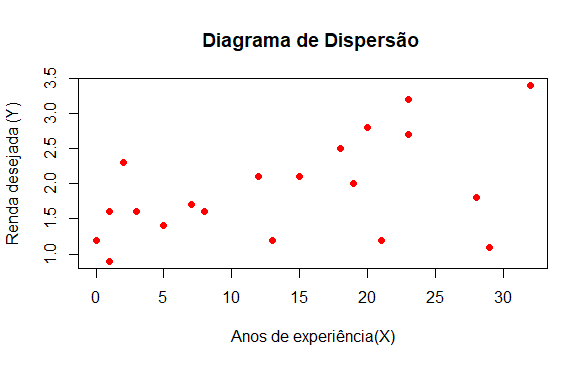
\includegraphics[width=0.8\textwidth]{Imagens/Graficos/Correlação 2-3.png} 
\end{figure}

\begin{lstlisting}
    plot(experiencia, renda,
+      main = "Diagrama de Dispersao ",
+      xlab = "Anos de experiencia(X)",
+      ylab = "Renda desejada (Y)",
+      pch = 19, 
+      col = "red")
\end{lstlisting}

Calculando o coeficiente de correlação
de Pearson:

Como temos as médias já calculadas da experiência (14) e da renda desejada (1.92) no item 2.1, agora podemos aplicar na fórmula calcular o somatório dos desvios.

\[r_{xy} = \frac{\sum{(x_i - \overline{x})(y_i-\overline{y})}}{\sqrt{\sum (x_i - \overline{x})^2 \sum(y_i-\overline{y})^2}}\]


\begin{table}[H]
    \centering
    \begin{tabular}{|c|c|c|c|c|}
        \hline
        \multicolumn{5}{|c|}{\textbf{Valores de Desvio (Experiência)}} \\
        \hline
        -12 & -6 & 7 & -13 & 1 \\
        -11 & 14 & -9 & -1 & 6 \\
        18 & 9 & -13 & -14 & 15 \\
        4 & 5 & -7 & -2 & 9 \\
        \hline
    \end{tabular}
    \caption{Desvios da Experiência}
    \label{tab:desvios_experiencia_h}
\end{table}

\begin{table}[H]
    \centering
    \begin{tabular}{|c|c|c|c|c|}
        \hline
        \multicolumn{5}{|c|}{\textbf{Valores de Desvio (Renda)}} \\
        \hline
        0.38 & -0.32 & -0.72 & -1.02 & 0.18 \\
        -0.32 & -0.12 & -0.52 & -0.72 & 0.88 \\
        1.48 & 0.78 & -0.32 & -0.72 & -0.82 \\
        0.58 & 0.08 & -0.22 & 0.18 & 1.28 \\
        \hline
    \end{tabular}
    \caption{Desvios da Renda }
    \label{tab:desvios_renda_h}
\end{table}

\vspace{5mm}

A partir dos desvios calculados na calculadora científica, utilizei o R como calculadora para calcular o somatório do numerador, dando resultado de 69.3.

\begin{lstlisting}
(-12 *0.38) + (-6*-0.32) + (7 * -0.72) + (-13 * -1.02) + (1*0.18) + (-11 * -0.32)+(14 * -0.12) + (-9 * -0.52) + (-1 * -0.72) + (6 * 0.88) + (18 * 1.48)+ (9 * 0.78)+ (-13 * -0.32) + (-14 * -0.72) + (15 * -0.82) + (4 * 0.58)+ (5 * 0.08) + (-7 * -0.22) + (-2 * 0.18) +(9 *1.28)

\end{lstlisting}

Para o denominador usando calculadora:


    \[\sum(experiência_i-\overline{experiencia})^2 =2004\]
    \[\sum(renda_i - \overline{renda})^2= 11.652\]


\[r_{experiência, renda} = \frac{69.3}{\sqrt{2004*11.652}}\]

\[r_{experiência, renda} = \frac{69.3}{\sqrt{23350.608}}\]

\[r_{experiência, renda} = \frac{69.3}{152.8090} = 0.453507\]


Valor calculado pela função em R:
\begin{lstlisting}
> r_coeficiente <- cor(experiencia, renda)
> r_coeficiente
[1] 0.4977672
\end{lstlisting}

\[Erro_{coeficiente} = |\frac{0.4977672 - 0.453507}{0.4977672} | *100 = 8.89\%\]

Analisando o gráfico de dispersão e o coeficiente de correlação calculado pela função em R, podemos perceber que existe uma correlação, porém, muito fraca para fazer uma inferência sobre experiência dos candidatos em relação à renda desejada, alguns candidatos com  15 ou até 30 anos de experiência desejam menos de 1.5 mil euros de renda, ou seja, não podemos afirmar que candidatos mais anos de experiência necessariamente desejam salários mais altos.


\textbf{\item[2.4] Resposta}: \\
Observando a tabela, conseguimos encontrar 4 candidatos que se enquadram nas exigências, segue a tabela abaixo:.

\begin{table}[H]
    \centering
    \label{tab_filtrada}
    \begin{tabular}{c l l c c}
        \toprule
        & \textbf{Idade} & \textbf{Nacionalidade} & \textbf{Renda (mil €)} & \textbf{Experiência (anos)} \\
        \midrule
        3  & 46 & Belga     & 1.2 & 21 \\
        7  & 51 & Francesa  & 1.8 & 28 \\
        9  & 39 & Italiana  & 1.2 & 13 \\
        15 & 52 & Italiana  & 1.1 & 29 \\
        \bottomrule
    \end{tabular}
    \caption{Candidatos com pelo menos 10 anos de experiência e renda desejada inferior a 2,0 mil euros.}
\end{table}

\textbf{\item[2.5] Resposta}: \\
Para obter essa representação transformarei os dados de idade e renda em médias para cada nacionalidade e agrupei em gráficos de barras.

\begin{figure}[H] 
    \centering 
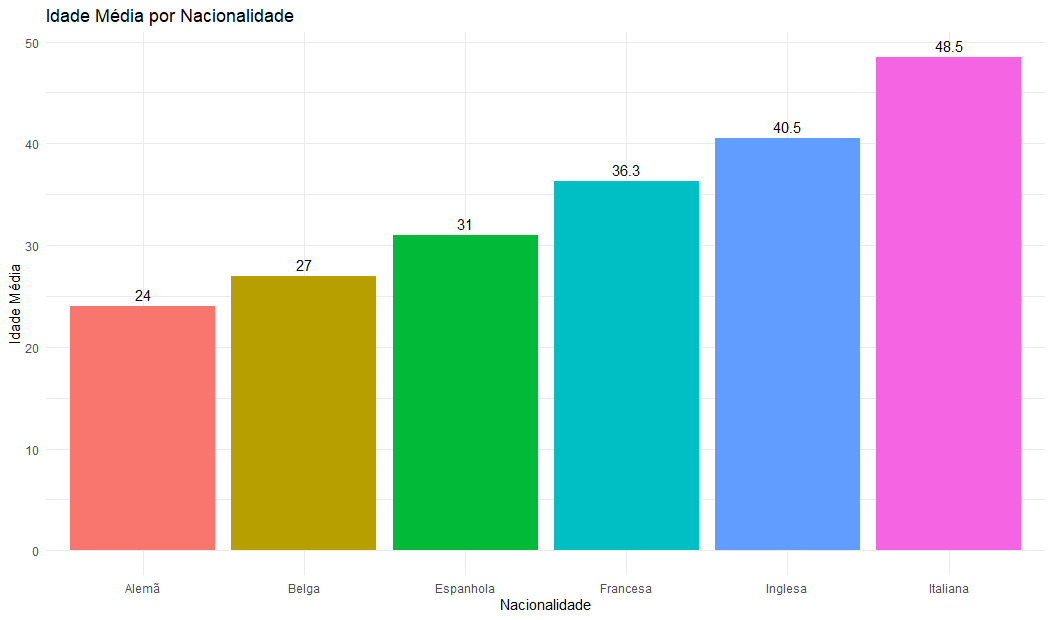
\includegraphics[width=0.8\textwidth]{Imagens/Graficos/Idade por nacionalidade.png} 
\end{figure}

\begin{lstlisting}
idade_media_nacionalidade <- curriculos %>%
  group_by(Nacionalidade) %>%
  summarise(Idade_Media = mean(Idade)) %>%
  ungroup() %>%
  arrange(desc(Idade_Media))

grafico_idade_media <- ggplot(idade_media_nacionalidade, aes(
  x = reorder(Nacionalidade, Idade_Media), 
  y = Idade_Media,
  fill = Nacionalidade
)) +
  geom_bar(stat = "identity") +
  geom_text(aes(label = round(Idade_Media, 1)), vjust = -0.5) +
  labs(
    title = "Idade Média por Nacionalidade",
    x = "Nacionalidade",
    y = "Idade Média"
  ) +
  theme_minimal() +
  theme(legend.position = "none")

print(grafico_idade_media)    
\end{lstlisting}

\begin{figure}[H] 
    \centering 
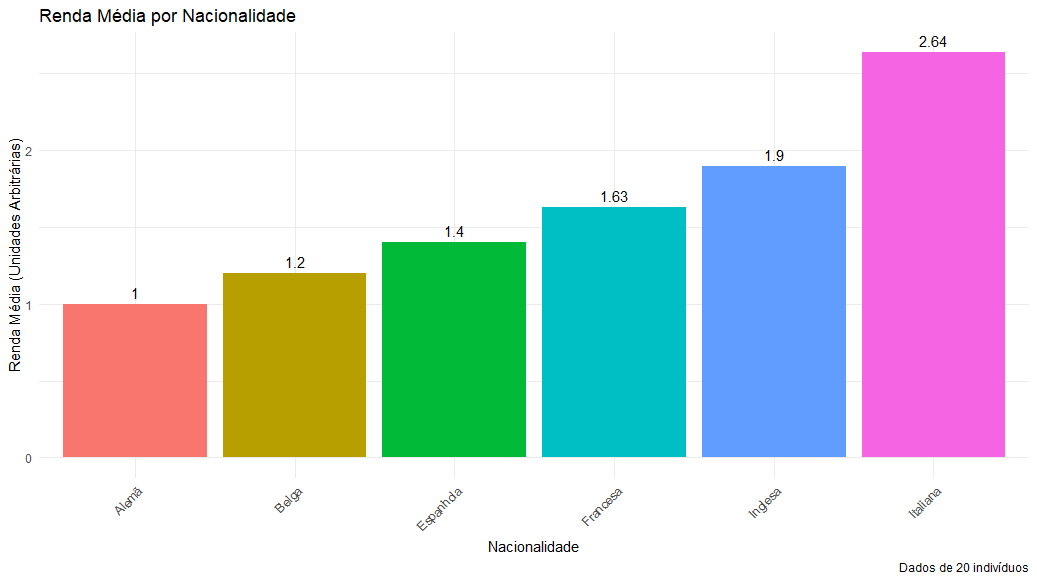
\includegraphics[width=0.8\textwidth]{Imagens/Graficos/renda por nacionalidade.png} 
\end{figure}

\begin{lstlisting}
renda_media_nacionalidade <- curriculos %>%
  group_by(Nacionalidade) %>%
  summarise(Renda_Media = mean(Renda)) %>% # Calcula a média da Renda
  ungroup() %>%
  arrange(desc(Renda_Media)) # Ordena o resultado para o gráfico


grafico_renda_media <- ggplot(renda_media_nacionalidade, aes(
  x = reorder(Nacionalidade, Renda_Media), 
  y = Renda_Media,
  fill = Nacionalidade 
)) +
  geom_bar(stat = "identity") +
  geom_text(aes(label = round(Renda_Media, 2)), vjust = -0.5) + 
  labs(
    title = "Renda Média por Nacionalidade",
    x = "Nacionalidade",
    y = "Renda Média (Unidades Arbitrárias)",
    caption = paste("Dados de", nrow(curriculos), "indivíduos")
  ) +
  theme_minimal() +
  theme(legend.position = "none", 
        axis.text.x = element_text(angle = 45, hjust = 1)) 

print(grafico_renda_media)
    
\end{lstlisting}

Após analisar os gráficos de barra podemos concluir que as maiores diferenças estão nos extremos do gráfico, tendo a nacionalidade Alemã como a nacionalidade composta em média por candidatos mais jovens do que as demais (24 anos) e a nacionalidade Italiana é composta em média por candidatos mais velhos (48.5 anos) do que as demais, tendo o dobro da média mais jovem. Com relação a renda desejada, a nacionalidade com a média mais jovem (Alemã) é a que em média deseja os menores salários, almejando apenas mil euros e a mais velha (Italiana) é a que deseja os maiores salários, almejando na casa de 2.64 mil euros.

\end{description}

\section{Questão} \label{sec:q3}
O conjunto de dados em anexo, {HW1\_bike\_sharing.csv}, refere-se ao processo de compartilhamento de bicicletas em uma cidade dos Estados Unidos. O conjunto contém as colunas descritas na Tabela 3. A variável season inclui as quatro estações do hemisfério norte: primavera, verão, outono e inverno. A variável weathersit representa quatro condições meteorológicas: ‘Céu limpo’, ‘Nublado’, ‘Chuva fraca’, ‘Chuva forte’. A variável temp é a temperatura normalizada em graus Celsius, ou seja, os valores foram divididos por 41 (valor máximo) 

\begin{table}[H]
    \centering
    % Define 4 colunas: a primeira centrada (c), as outras três alinhadas à esquerda (l)
    \begin{tabular}{c l l l}
        \toprule
        \textbf{TAG} & \textbf{DESCRIÇÃO} & \textbf{DESCRIPTION} \\
        \midrule
        instant & Índice de registro & \textcolor{blue}{Record index} \\
        dteday & Data da observação & \textcolor{blue}{Date of observation} \\
        season & Estação do ano & \textcolor{blue}{Season} \\
        weathersit & Condições meteorológicas & \textcolor{blue}{Weather conditions} \\
        temp & Temperatura em \textdegree C (normalizada) & \textcolor{blue}{Temperature in \textdegree C (normalised)} \\
        casual & Número de usuários casuais & \textcolor{blue}{Number of casual users} \\
        registered & Número de usuários registrados & \textcolor{blue}{Number of registered users} \\
        \bottomrule
    \end{tabular}
    \caption{Variáveis do conjunto HW1\_bike\_sharing (questão \ref{sec:q3}).}
    \label{tab:variaveis_bike}
\end{table}

\begin{enumerate}[leftmargin=*]
\item Carregue o conjunto de dados \texttt{HW1\_bike\_sharing.csv}  no R. Classifique as variáveis quanto ao tipo (categórica ou numérica), identifique o número total de observações e as datas de início e fim da amostra.

\item Calcule medidas de tendência central (média, mediana) e os quartis para cada característica numérica relevante. Apresente os resultados em uma tabela com título
apropriado. Comente os principais pontos

\item Atribua os níveis correspondentes às variáveis season e weathersit. Construa gráficos de barras para ambas. Qual estação do ano apresenta maior número de usuários? O uso de bicicletas depende da estação? Qual é a condição climática mais favorável para o uso do sistema?

\item Calcule o número total de usuários por dia, somando casual e registered. Converta
a variável temp para temperatura real (multiplicando por 41). Em seguida, construa os gráficos de séries temporais para temperatura e número total de usuários. Essas séries apresentam tendência semelhante?

\end{enumerate}

\subsection*{Solução da questão} 					

\subsubsection*{Descrição da atividade}
Essa ultima atividade visa introduzir o ultimo conteúdo de estatística descritiva restante a ser abordado por este homework, sendo este, os tipos de dados e suas diferentes formas de interpretação.


\subsubsection*{Base Teórica Questão 3:} 

\begin{itemize}
\item[]

\subsubsection*{Tipos de dados - base teórica} 

\item \text{Dados quantitativos:} são quaisquer dados que medem ou estão associados a medições numéricas de alguma quantidade.
    \begin{itemize}
        \item \text{Variáveis Quantitativas Discretas:} Assumem valores em um conjunto finito ou infinito contável de números.
        \item \text{Variáveis Quantitativas Contínuas:} Dados contínuos assumem valores em um intervalo de números. Eles também são conhecidos como dados de escala, dados de intervalo ou dados de medição
    \end{itemize}
    \item \text{Dados qualitativos:} são quaisquer tipos de dados que não são numéricos ou não representam quantidades numéricas.
    \begin{itemize}
        \item \text{Variáveis Qualitativas Nominais:} Tem níveis que correspondem aos nomes das categorias, e não há nenhuma ordenação implícita
        \item \text{Variáveis Qualitativas Ordinais:} Tem uma estrutura ordenada para os níveis de fatores subjacentes
    \end{itemize}

    
\end{itemize}


\begin{description}[leftmargin=*] 

\item[3.1] \textbf{ Resposta}: \\
o conjunto de dados possui sete variáveis, sendo elas:
\begin{itemize}
    \item instant (Categórico)
    \item dteday (Categórico)
    \item season (Categórico)
    \item weathersit (Categórico)
    \item temp (Numérico contínuo)
    \item casual (Numérico ordinário)
    \item registered (Numérico ordinário)
\end{itemize}

Importando os dados para o arquivo R:

\begin{lstlisting}
> dados <- read.csv("Estatistica\\1-HomeWorks\\HW-1\\code\\HW1_bike_sharing.csv")
> View(dados)
\end{lstlisting}

Com os dados devidamente importados, podemos observar através de funções em R ou observando a tabela que o conjunto possui 731 observações, que se iniciam em 2011-01-01 e vão até 2012-12-31 (aaaa/mm/dd).

\begin{lstlisting}
> n_dados <- nrow(dados)
> n_dados
[1] 731
> data_inicio <- min(dados$dteday)
> data_inicio
[1] "2011-01-01"
> data_fim <- max(dados$dteday)
> data_fim
[1] "2012-12-31"
\end{lstlisting}

\textbf{\item[3.2] Resposta}: \\
Calcularemos as medidas de tendência central e os quartis para os dados numéricos que são: temp, casual e registered.

\vspace{5mm}

Usando o R para calcular as medidas de tendência central com o seguinte código:

\vspace{5mm}

\item \textbf{temp}
\begin{lstlisting}
> media_temp <- mean(dados$temp)
> media_temp 
[1] "20.3112175102599"
> mediana_temp <- median(dados$temp)
> mediana_temp
[1] "20.4"
> Q1_temp <- quantile(dados$temp, 0.25)
> Q1_temp      
 25% 
13.8
> Q3_temp <- quantile(dados$temp, 0.75)
> Q3_temp      
 75% 
26.9
\end{lstlisting}

\vspace{5mm}

\item \textbf{casual}
\begin{lstlisting}
> media_casual <- mean(dados$casual)
> media_casual
[1] 848.1765
> mediana_casual <- median(dados$casual)
> mediana_casual
[1] 713
> Q1_casual <- quantile(dados$casual, 0.25)
> Q1_casual
  25% 
315.5
> Q3_casual <- quantile(dados$casual, 0.75)
> Q3_casual
 75% 
1096
\end{lstlisting}

\vspace{5mm}

\item \textbf{registered}
\begin{lstlisting}
> media_registered <- mean(dados$registered)
> media_registered  
[1] 3656.172
> mediana_registered <- median(dados$registered)
> mediana_registered 
[1] 3662
> Q1_registered <- quantile(dados$registered, 0.25)
> Q1_registered
 25% 
2497
> Q3_registered <- quantile(dados$registered, 0.75)
> Q3_registered
 75% 
4776.5
\end{lstlisting}

\begin{table}[H]
    \centering
    \label{tab:resumo_estatistico}
    \begin{tabular}{l c c c c}
        \toprule
        \textbf{Variável} & \textbf{Média} & \textbf{Mediana} & \textbf{Q1 (25\%)} & \textbf{Q3 (75\%)} \\
        \midrule
        temp        & 20.31 & 20.4  & 13.8   & 26.9    \\
        casual      & 848.18 & 713   & 315.5  & 1096    \\
        registered  & 3656.17 & 3662 & 2497  & 4776.5  \\
        \bottomrule
    \end{tabular}
    \caption{Resumo estatístico das variáveis `temp`, `casual` e `registered`.}
\end{table}



\textbf{\item[3.3] Resposta}: \\

Importamos o conjunto de dados e atribuindo os seguintes níveis ao fator season (estação):
\begin{itemize}
    \item 1 = primavera
    \item 2 = verão
    \item 3 = outono 
    \item 4 = inverno
\end{itemize}

\begin{lstlisting}
dados <- read.csv("Estatistica\\1-HomeWorks\\HW-1\\code\\HW1_bike_sharing.csv")

dados$season <- factor(
  x = dados$season,
  levels = c(1, 2, 3, 4),              
  labels = c("Primavera", "Verão", "Outono", "Inverno")
)

\end{lstlisting}


Atribuindo os seguintes níveis ao fator weathersit (tempo):
\begin{itemize}
    \item 1 = Céu limpo
    \item 2 = Nublado
    \item 3 = Chuva fraca 
    \item 4 = Chuva forte
\end{itemize}


\begin{lstlisting}
dados$weathersit <- factor(
  x = dados$weathersit,
  levels = c(1,2,3,4),
  labels = c("Céu limpo", "Nublado", "Chuva fraca", "Chuva forte")
)

\end{lstlisting}

Plotando o gráfico das estações:

\begin{figure}[H] 
    \centering 
    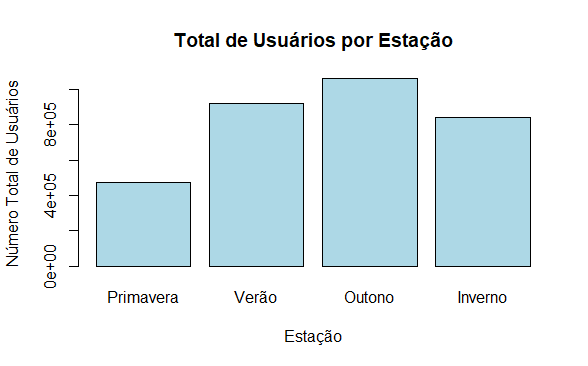
\includegraphics[width=0.8\textwidth]{Imagens/Graficos/Distribuição estação.png} 
\end{figure}

Criamos um dataframe de season e usuários totais que é a soma dos usuários casuais e dos registrados, depois fazendo uma agregação de total de usuários com as estações, após isso podemos plotar o gráfico utilizando a função barplot.

\begin{lstlisting}
season_usuarios <- data.frame(
  Season = dados$season,
  Usuarios = dados$casual + dados$registered
)

sumario_estacoes <- aggregate(
  Usuarios ~ Season,             
  data = season_usuarios,
  FUN = sum
)


barplot(
  sumario_estacoes$Usuarios,
  names.arg = sumario_estacoes$Season, 
  main = "Total de Usuários por Estação",
  xlab = "Estação",
  ylab = "Número Total de Usuários",
  border = "black",
  col = "lightblue"
)

\end{lstlisting}

Plotando o gráfico do clima:

\begin{figure}[H] 
    \centering 
    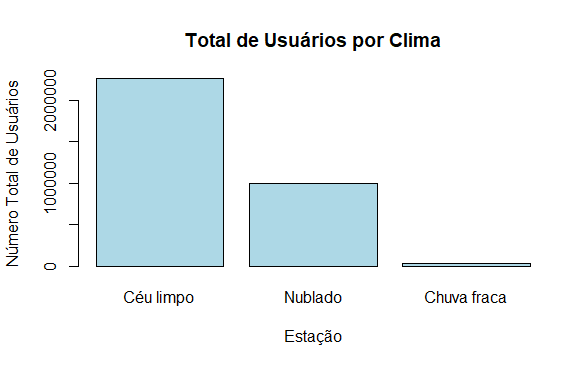
\includegraphics[width=0.8\textwidth]{Imagens/Graficos/Distribuição clima.png} 
\end{figure}

Criamos um dataframe de weathersit e usuários totais que é a soma dos usuários casuais e dos registrados, depois fazendo uma agregação de total de usuários com os climas, após isso podemos plotar o gráfico utilizando a função barplot.

\begin{lstlisting}
weathersit_usuarios <- data.frame(
  Weathersit = dados$weathersit,
  Usuarios = dados$casual + dados$registered
)

sumario_weathersit <- aggregate(
  Usuarios ~ Weathersit,             
  data = weathersit_usuarios,
  FUN = sum
)


barplot(
  sumario_weathersit$Usuarios,
  names.arg = sumario_weathersit$Weathersit, 
  main = "Total de Usuários por Clima",
  xlab = "Estação",
  ylab = "Número Total de Usuários",
  border = "black",
  col = "lightblue"
)
\end{lstlisting}

Podemos constatar que a estação que possui maior número de usuários é o outono, o uso das bicicletas depende das estações pois durante a primavera a frequência de uso é menos da metade da estação de outono e a condição climática mais favorável é a de céu limpo.

\textbf{\item[3.4] Resposta}: \\
Usaremos o R para de cara já fazer as alterações que se pede (converter a temperatura e total de usuários):

\begin{lstlisting}
dados <- dados %>%
  mutate(temp_C = temp * 41,
         total_users = casual + registered)
)
\end{lstlisting}

Em seguida, com os dados já modificados, criamos o gráfico de séries temporais da temperatura.

\begin{lstlisting}
plot(dados$dteday, dados$temp_C, type = "l", col = "red",
     xlab = "Data", ylab = "Temperatura (°C)",
     main = "Série Temporal da Temperatura")
\end{lstlisting}

Gráfico de séries temporais da temperatura:

\begin{figure}[H] 
    \centering 
    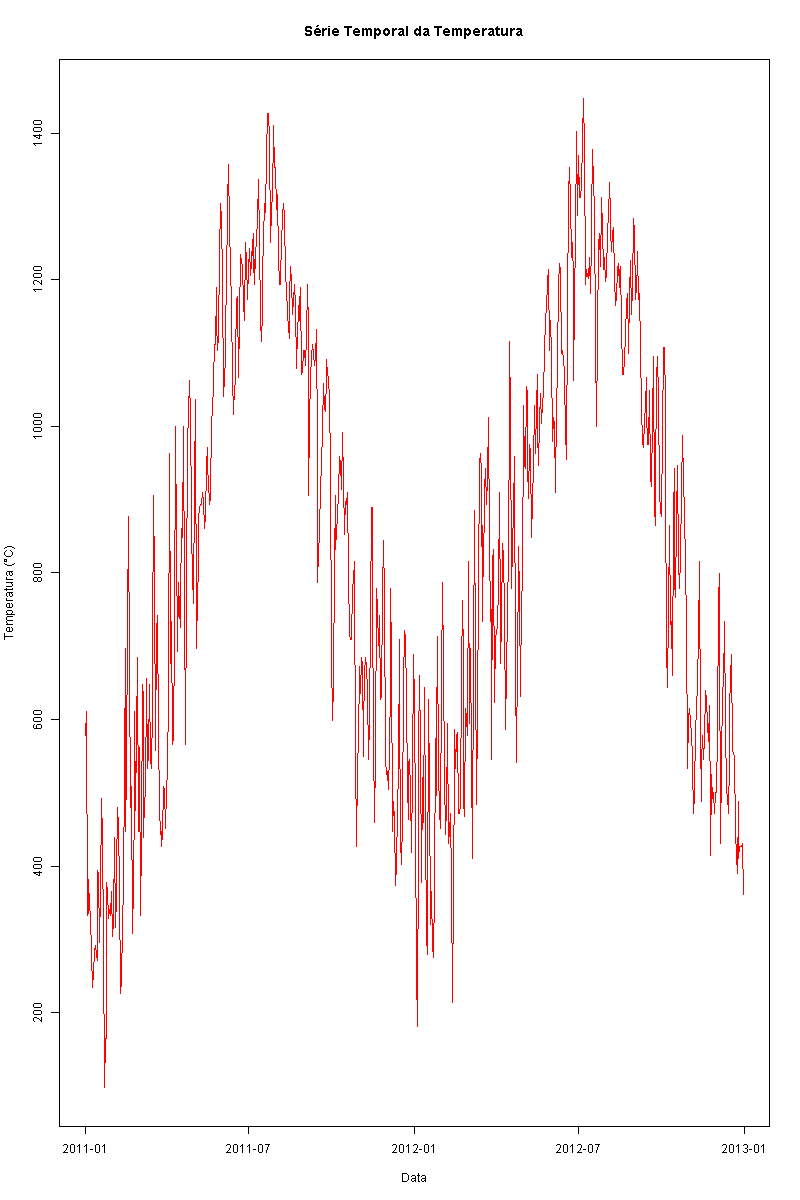
\includegraphics[width=0.4\textwidth]{Imagens/Graficos/serie_temporal_temperatura_3-4} 
\end{figure}

Logo após, criamos o gráfico de séries temporais dos usuários totais.

\begin{lstlisting}
plot(dados$dteday, dados$total_users, type = "l", col = "blue",
     xlab = "Data", ylab = "Total de Usuários",
     main = "Série Temporal do Número Total de Usuários")
\end{lstlisting}

Gráfico de séries temporais dos usuários totais.

\begin{figure}[H] 
    \centering 
    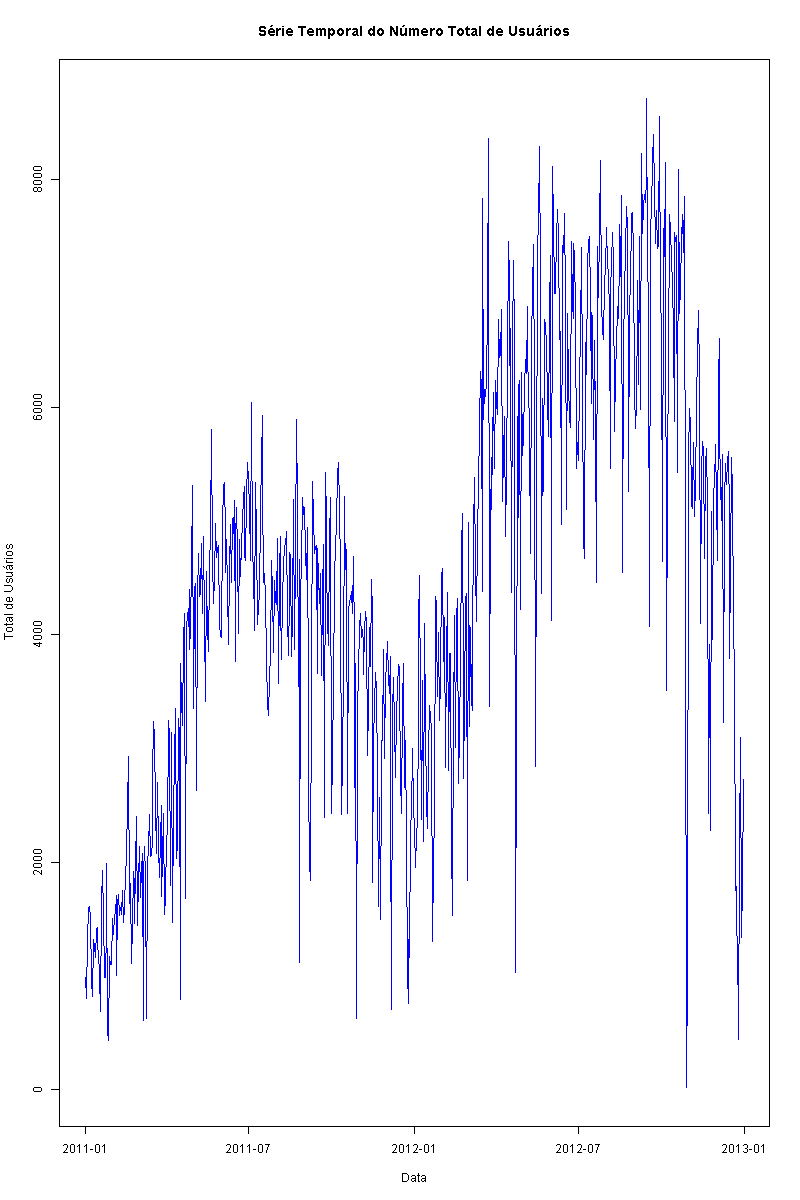
\includegraphics[width=0.4\textwidth]{Imagens/Graficos/serie_temporal_usuarios_3-4} 
\end{figure}

Por fim, para facilitar a minha análise, eu criei um código em R para juntar os dois gráficos e deixar mais visível a comparação deles.

\begin{lstlisting}
plot(dados$dteday, dados$total_users, type = "l", col = "blue",
     xlab = "Data", ylab = "Total de Usuários",
     main = "Comparação: Temperatura vs Total de Usuários")
par(new = TRUE)
plot(dados$dteday, dados$temp_C, type = "l", col = "red",
     axes = FALSE, xlab = "", ylab = "")
axis(side = 4)
mtext("Temperatura (°C)", side = 4, line = 3)
legend("topleft", legend = c("Total de Usuários", "Temperatura (°C)"),
       col = c("blue", "red"), lty = 1)
\end{lstlisting}

Gráfico para comparação.

\begin{figure}[H] 
    \centering 
    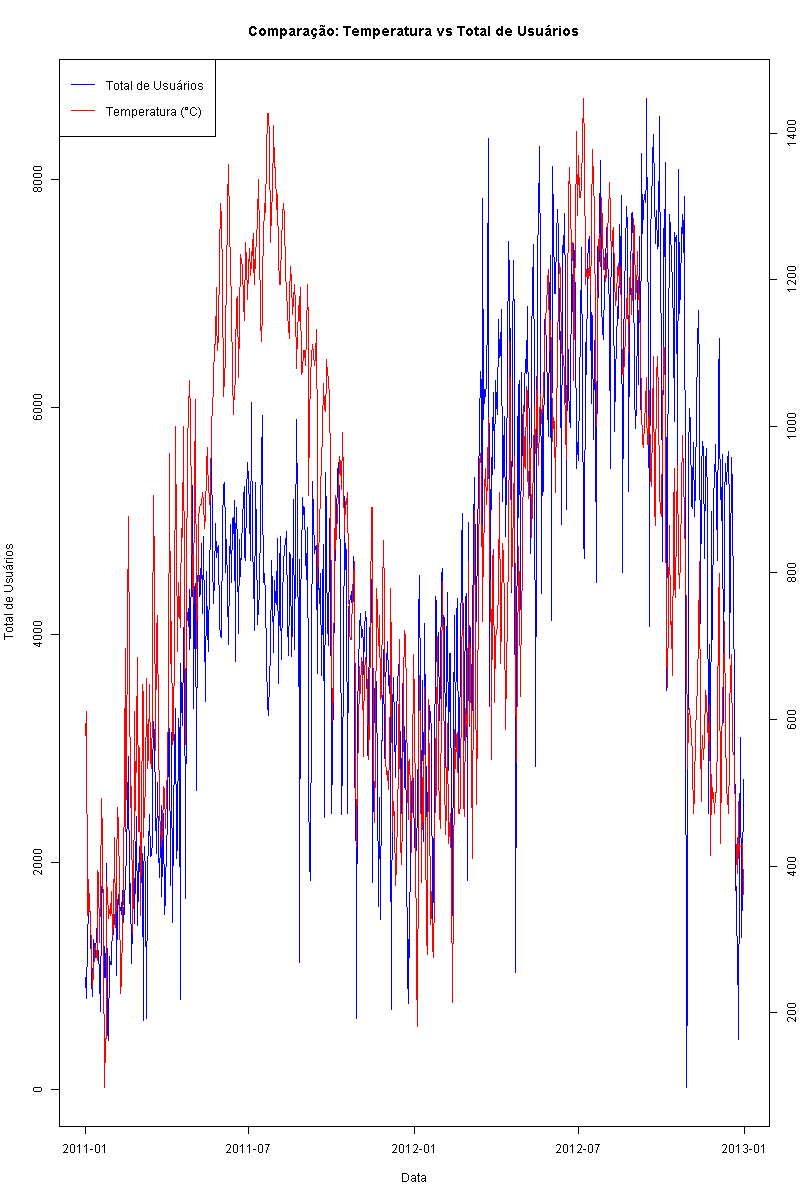
\includegraphics[width=0.4\textwidth]{Imagens/Graficos/serie_temporal_comparação_3-4.png} 
\end{figure}

\end{description}

\newpage
\begin{appendices}


\end{appendices}

\end{document}
